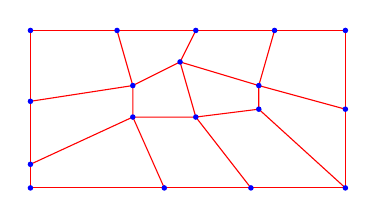
\begin{tikzpicture}
	\draw[red] (0,0) rectangle (4,2);
	\draw[red] (0,1.1)--(1.3,1.3)--(1.9,1.6)--(2.9,1.3)--(4,1);
	\draw[red] (0,.3) --(1.3,.9) --(2.1,.9) --(2.9,1);
	\draw[red] (1.1,2)--(1.3,1.3)--(1.3,.9)-- (1.7,0);
	\draw[red] (2.1,2)--(1.9,1.6)--(2.1,.9)-- (2.8,0);
	\draw[red] (3.1,2)--(2.9,1.3)--(2.9,1) -- (4,0);
		
	\foreach \p in {(0,0),(1.7,0),(2.8,0),(4,0),(4,1),(4,2),(3.1,2),(2.1,2),
		(1.1,2),(0,2),(0,1.1),(0,.3),(1.3,1.3),(1.3,.9),(1.9,1.6),(2.1,.9),
	 	(2.9,1.3),(2.9,1)}	
		\fill[blue] \p circle (1pt);
\end{tikzpicture}